\definecolor{customblue}{HTML}{155DFC}
\definecolor{customred}{HTML}{E7180B}

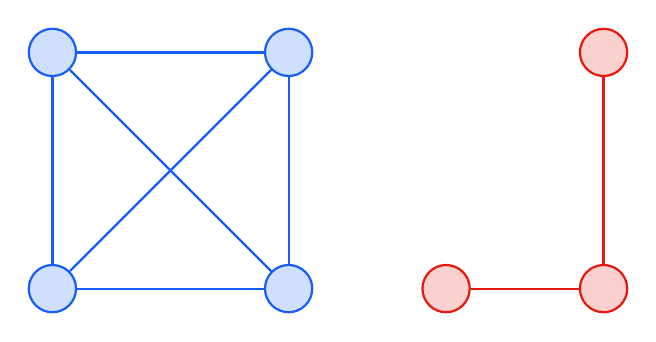
\begin{tikzpicture}[scale=1,auto=left]
  % Estilos para cada componente
  \tikzset{
    blue_node/.style={circle,fill=customblue!20,draw=customblue,thick,minimum size=6mm},
    red_node/.style={circle,fill=customred!20,draw=customred,thick,minimum size=6mm}
  }

  % Componente izquierda (Grafo completo K_4) en azul
  \node[blue_node] (n1) at (0,3) {};
  \node[blue_node] (n2) at (3,3) {};
  \node[blue_node] (n3) at (0,0) {};
  \node[blue_node] (n4) at (3,0) {};

  \foreach \from/\to in {n1/n2,n1/n3,n1/n4,n2/n3,n2/n4,n3/n4}
    \draw[customblue,thick] (\from) -- (\to);

  % Componente derecha (Camino P_3) en rojo
  \node[red_node] (n5) at (5,0) {};
  \node[red_node] (n6) at (7,0) {};
  \node[red_node] (n7) at (7,3) {};

  \foreach \from/\to in {n5/n6,n6/n7}
    \draw[customred,thick] (\from) -- (\to);
\end{tikzpicture}
